\documentclass{beamer}
\mode<presentation>{
  \usetheme{Boadilla}
  \usefonttheme[onlylarge]{structurebold}
  \usefonttheme[stillsansseriflarge]{serif}
  \setbeamerfont*{frametitle}{size=\normalsize,series=\bfseries}
  % \setbeamertemplate{navigation symbols}{}
  \setbeamercovered{transparent}
}
\usepackage[english]{babel}
\usepackage[latin1]{inputenc}
\usepackage{times}
\usepackage[T1]{fontenc}
\usepackage{amsmath}
\usepackage{amssymb}
\usepackage{esint}
\usepackage{hyperref}
\usepackage{tikz}
\usepackage{xkeyval}
\usepackage{xargs}
\usepackage{verbatim}
\usepackage{listings}
\usepackage{multimedia}
\usetikzlibrary{
  arrows,
  calc,
  decorations.pathmorphing,
  decorations.pathreplacing,
  decorations.markings,
  fadings,
  positioning,
  shapes
}

\mode<handout>{
  \usepackage{pgfpages}
  \pgfpagesuselayout{4 on 1}[a4paper,landscape,border shrink=5mm]
  \setbeamercolor{background canvas}{bg=black!10}
}

\newcommand\pgfmathsinandcos[3]{%
  \pgfmathsetmacro#1{sin(#3)}%
  \pgfmathsetmacro#2{cos(#3)}%
}
\newcommand\LongitudePlane[3][current plane]{%
  \pgfmathsinandcos\sinEl\cosEl{#2} % elevation
  \pgfmathsinandcos\sint\cost{#3} % azimuth
  \tikzset{#1/.estyle={cm={\cost,\sint*\sinEl,0,\cosEl,(0,0)}}}
}
\newcommand\LatitudePlane[3][current plane]{%
  \pgfmathsinandcos\sinEl\cosEl{#2} % elevation
  \pgfmathsinandcos\sint\cost{#3} % latitude
  \pgfmathsetmacro\yshift{\cosEl*\sint}
  \tikzset{#1/.estyle={cm={\cost,0,0,\cost*\sinEl,(0,\yshift)}}} %
}
\newcommand\DrawLongitudeCircle[2][1]{
  \LongitudePlane{\angEl}{#2}
  \tikzset{current plane/.prefix style={scale=#1}}
  % angle of "visibility"
  \pgfmathsetmacro\angVis{atan(sin(#2)*cos(\angEl)/sin(\angEl))} %
  \draw[current plane] (\angVis:1) arc (\angVis:\angVis+180:1);
  \draw[current plane,dashed] (\angVis-180:1) arc (\angVis-180:\angVis:1);
}
\newcommand\DrawLatitudeCircleArrow[2][1]{
  \LatitudePlane{\angEl}{#2}
  \tikzset{current plane/.prefix style={scale=#1}}
  \pgfmathsetmacro\sinVis{sin(#2)/cos(#2)*sin(\angEl)/cos(\angEl)}
  % angle of "visibility"
  \pgfmathsetmacro\angVis{asin(min(1,max(\sinVis,-1)))}
  \draw[current plane,decoration={markings, mark=at position 0.6 with {\arrow{<}}},postaction={decorate},line width=.6mm] (\angVis:1) arc (\angVis:-\angVis-180:1);
  \draw[current plane,dashed,line width=.6mm] (180-\angVis:1) arc (180-\angVis:\angVis:1);
}
\newcommand\DrawLatitudeCircle[2][1]{
  \LatitudePlane{\angEl}{#2}
  \tikzset{current plane/.prefix style={scale=#1}}
  \pgfmathsetmacro\sinVis{sin(#2)/cos(#2)*sin(\angEl)/cos(\angEl)}
  % angle of "visibility"
  \pgfmathsetmacro\angVis{asin(min(1,max(\sinVis,-1)))}
  \draw[current plane] (\angVis:1) arc (\angVis:-\angVis-180:1);
  \draw[current plane,dashed] (180-\angVis:1) arc (180-\angVis:\angVis:1);
}
\newcommand\coil[1]{
  {\rh * cos(\t * pi r)}, {\apart * (2 * #1 + \t) + \rv * sin(\t * pi r)}
}
\makeatletter
\define@key{DrawFromCenter}{style}[{->}]{
  \tikzset{DrawFromCenterPlane/.style={#1}}
}
\define@key{DrawFromCenter}{r}[1]{
  \def\@R{#1}
}
\define@key{DrawFromCenter}{center}[(0, 0)]{
  \def\@Center{#1}
}
\define@key{DrawFromCenter}{theta}[0]{
  \def\@Theta{#1}
}
\define@key{DrawFromCenter}{phi}[0]{
  \def\@Phi{#1}
}
\presetkeys{DrawFromCenter}{style, r, center, theta, phi}{}
\newcommand*\DrawFromCenter[1][]{
  \setkeys{DrawFromCenter}{#1}{
    \pgfmathsinandcos\sint\cost{\@Theta}
    \pgfmathsinandcos\sinp\cosp{\@Phi}
    \pgfmathsinandcos\sinA\cosA{\angEl}
    \pgfmathsetmacro\DX{\@R*\cost*\cosp}
    \pgfmathsetmacro\DY{\@R*(\cost*\sinp*\sinA+\sint*\cosA)}
    \draw[DrawFromCenterPlane] \@Center -- ++(\DX, \DY);
  }
}
\newcommand*\DrawFromCenterText[2][]{
  \setkeys{DrawFromCenter}{#1}{
    \pgfmathsinandcos\sint\cost{\@Theta}
    \pgfmathsinandcos\sinp\cosp{\@Phi}
    \pgfmathsinandcos\sinA\cosA{\angEl}
    \pgfmathsetmacro\DX{\@R*\cost*\cosp}
    \pgfmathsetmacro\DY{\@R*(\cost*\sinp*\sinA+\sint*\cosA)}
    \draw[DrawFromCenterPlane] \@Center -- ++(\DX, \DY) node {#2};
  }
}
\makeatother

% not mandatory, but I though it was better to set it blank
\setbeamertemplate{headline}{}
\def\beamer@entrycode{\vspace{-\headheight}}

\tikzstyle{snakearrow} = [decorate, decoration={pre length=0.2cm,
  post length=0.2cm, snake, amplitude=.4mm,
  segment length=2mm},thick, ->]

%% document-wide tikz options and styles

\tikzset{%
  % >=latex, % option for nice arrows
  inner sep=0pt,%
  outer sep=2pt,%
  mark coordinate/.style={inner sep=0pt,outer sep=0pt,minimum size=3pt,
    fill=black,circle}%
}
\tikzset{
  % Define standard arrow tip
  >=stealth',
  % Define style for boxes
  punkt/.style={
    rectangle,
    rounded corners,
    draw=black, very thick,
    text width=8em,
    minimum height=2.5em,
    text centered},
}
\makeatletter
\newbox\@backgroundblock
\newenvironment{backgroundblock}[2]{%
  \global\setbox\@backgroundblock=\vbox\bgroup%
  \unvbox\@backgroundblock%
  \vbox to0pt\bgroup\vskip#2\hbox to0pt\bgroup\hskip#1\relax%
}{\egroup\egroup\egroup}
\addtobeamertemplate{background}{\box\@backgroundblock}{}
\makeatother

% \def\timeleft{15:00->14:55}

\title[Na \textbf{and} Cs update]{\only<1>{NaCs update}\only<2->{Na {\huge AND} Cs update}}
\date{November 4, 2016}
\author{Yichao Yu}
\institute{Ni Group/Harvard}

\begin{document}

\begin{frame}{}
  \titlepage
\end{frame}

% \begin{frame}{}
%   \tableofcontents
% \end{frame}

% Good Cs Raman cooling result. Work on Na again.
% Haven't been talking about Na for a few month.
% Not only Na but to make sure Na and Cs can work together.

\begin{frame}{Load Na and Cs at the same time}
  \begin{block}{Overlap Na and Cs MOT}
    \begin{itemize}
    \item<2-> Retro beam collimation\\
      \visible<3->{\textbf{Expand} retro beam by $5\sim20\%$}
    \item<4-> Align the MOT beams using the MOT itself
    \end{itemize}
  \end{block}
  \visible<5-> {
    \begin{block}{Result}
      \begin{itemize}
      \item<6-> Na AND Cs MOT at the same B field.
      \item<7-> $50\%$ Na loading rate.
      \item<8-> $<1$ second Na loading time.
      \item<9-> Na live loading.
      \end{itemize}
    \end{block}
  }
\end{frame}

\begin{frame}{Load Na and Cs at the same time}
  \begin{block}{Load single atoms at the same time}
    \begin{itemize}
    \item<2-> Separate trap beams
    \end{itemize}
  \end{block}
  \visible<3-> {
    \begin{center}
      \begin{tikzpicture}
        \visible<3> {
          % Na beams
          \draw[->, blue, line width=1.5] (-1.2, -1.5) -- (-1.2, -0.8);
          \draw[->, blue, line width=1.5] (-0.8, -1.5) -- (-0.8, -0.8);
          \draw[blue, line width=1.5] (-1.2, -0.9) -- (-1.2, -0.2);
          \draw[blue, line width=1.5] (-0.8, -0.9) -- (-0.8, 0.2);
          \path (-1, -1.5) node[blue, below] {\textbf{\LARGE Na}};

          % Cs beams
          \draw[->, red, line width=1.5] (-2.5, -0.2) -- (-1.8, -0.2);
          \draw[->, red, line width=1.5] (-2.5, 0.2) -- (-1.8, 0.2);
          \draw[red, line width=1.5] (-1.9, -0.2) -- (-1.2, -0.2);
          \draw[red, line width=1.5] (-1.9, 0.2) -- (-0.8, 0.2);
          \path (-2.5, 0) node[red, left] {\textbf{\LARGE Cs}};

          % Combined beams
          \draw[orange, line width=1.5] (-1.2, -0.2) -- (0, -0.2) -- (3, 0.8) -- (4, 0.8);
          \draw[orange, line width=1.5] (-0.8, 0.2) -- (0, 0.2) -- (3, -0.8) -- (4, -0.8);
          \draw[orange, line width=1.5] (6.8, 0.6) -- (7.5, 0) -- (6.8, -0.6);

          % Telescope
          \draw[<->, line width=1.5] (0, -0.3) -- (0, 0.3);
          \draw[<->, line width=2] (3, -1) -- (3, 1);

          % Dichroic
          \draw[cyan, line width=2] (-1.5, -0.5) -- (-0.5, 0.5);

          % Objective
          \draw[line width=2] (4, -1) rectangle (6.5, 1);
          \draw[line width=2] (6.5, -1) -- (6.8, -0.7) -- (6.8, 0.7) -- (6.5, 1);
          \path (4.1, 0) node[right] {\textbf{\Large Objective}};
        }
        \visible<4> {
          \path (1.9, -0.8) node {
            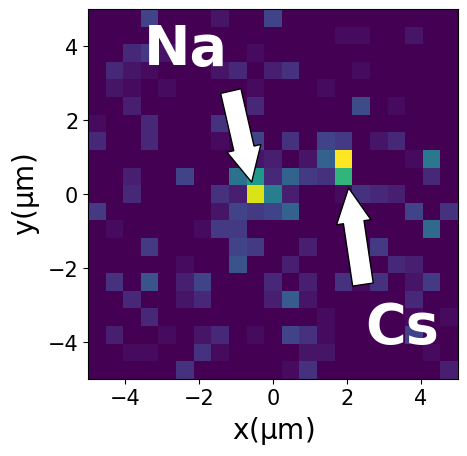
\includegraphics[width=5cm]{../../experiments/nacs_atoms/imgs/single_viridis.png}
            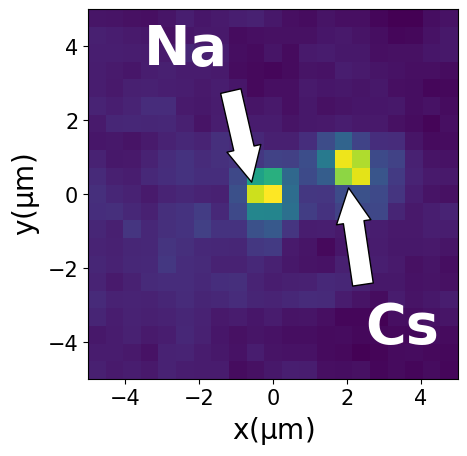
\includegraphics[width=5cm]{../../experiments/nacs_atoms/imgs/avg_viridis.png}
          };
        }
      \end{tikzpicture}
    \end{center}
  }
\end{frame}

\begin{frame}{Other Na improvements}
  \visible<+->{
    \begin{block}{}
      \begin{itemize}
      \item<+-> Temperature stability
      \item<+-> Optimize molasses cooling
      \item<+-> Optimize optical pumping
      \end{itemize}
    \end{block}
  }
\end{frame}

\begin{frame}{}
\end{frame}

\end{document}
